\documentclass[times, twoside, watermark]{style}
\usepackage{blindtext}
\usepackage{empheq}
\usepackage{tikz}
\usepackage{pgfplots} 
\usepackage{subcaption}
\usepackage{amsmath}
\usepackage{cases}
\usepackage{algorithmicx}
\usepackage{algorithm}
\usepackage{algpseudocode}

\leadauthor{Paul-Antoine LE TOLGUENEC} 

\begin{document}

\title{Point-to-Point Navigation with Deep Reinforcement Learning }
\shorttitle{ Deep Reinforcement Learning}

% Use letters for affiliations, numbers to show equal authorship (if applicable) and to indicate the corresponding author
\author[1,\Letter]{ Paul-Antoine Le Tolguenec}

\affil[1]{ENSTA Bretagne, Brest}

\maketitle

%TC:break Abstract
%the command above serves to have a word count for the abstract
\begin{abstract}
    Nowadays the problem of the autonomous vehicle is one of the most developed subjects in the world of research. 
    Although there are different methods, methods based on deep learning are more and more used in this field. 
    This article illustrates a solution based on Deep Reinforcement Learning.
\end {abstract}
%TC:break main
%the command above serves to have a word count for the abstract

\begin{keywords}
Deep learning | Reinforcement | Control | Autonomous car
\end{keywords}

\begin{corrauthor}
%\texttt{r.henriques{@}ucl.ac.uk}
paul-antoine.le\textunderscore tolguenec\at ensta-bretagne.org
\end{corrauthor}

\maketitle

\section*{Introduction}
In recent years, mobile robotics has experienced unprecedented growth. Most of the methods concerning trajectory estimation are based on automatic laws.
A very robust method is the linearizing loop control method. But in some cases this method has to be reworked, because it has to be linearised around a working point or other. 
Another very robust method is that of potential fields, since it also allows to avoid certain obstacles that could appear spontaneously on the way to the robot. 
But for this type of method it is often necessary to implement other layers that allow to find the path to reach a point in the defined space. 
Most of the time it is also necessary to develop a finite state machine to manage the high level of the robot. 
Usual methods are therefore very time-consuming to implement and can lead to mistakes. Moreover, once the control of the robot is set up, optimisation is difficult.
With the progress of deep learning, a new control approach has emerged: deep reinforcement learning.
The advantage of this method is that once the method is set up it can be generalised to many problems and it is only necessary to change certain parameters. Also this method is permanently optimized.
In this article, I expose my work which has allowed me to train a model to make decisions to orientate a car so that it is able to go from point A to point B as quickly as possible by avoiding objects \cite{avoidance} that appear as they go along.
To train the model I use the A2C (Advantage Actor Critic) algorithm which uses the principle of reinforcement learning.
Part II illustrates the modelling I have carried out and within which I have trained the network. Part III presents the implementation of the method (network architecture, theory ...).
Finally, part IV illustrates the experimentation phase.

\section{Modelisation}
    \subsection{Formalisme}
    The objective of our work is to automate a car so that it is able to go from point A to point B while avoiding obstacles.
    The kinematics of the car is modelled by the following equations:
        \begin{equation}
            \label{eqn:constrains}
            \begin{cases}
                (\mathit{i}) & \dot{x} = v\cos{\phi} \\
                (\mathit{ii}) & \dot{x} = v\sin{\phi} \\
                (\mathit{iii}) & \phi=u_{\pi_{\theta}} \\
                (\mathit{iv}) &  v = k \\
               
            \end{cases}
        \end{equation}
    At first, I tried to control only the steering angle of the car. Thus $u_{\pi_{\theta}}$ represents the $\phi$ output taken via a policy $\pi_{\theta}$.
    The robot is also equipped with three sonars, one frontal and two lateral, which allow to visualize its environment.

    \subsection{Simulation}
    Once the kinematics were defined, I had to simulate the robot and obtain a visual rendering. I used the Kivy library of python. 
    Kivy is a free and open source Python framework for developing mobile apps and other multitouch application software with a natural user interface.
    The objective was to have a visual rendering of the robot's evolution, but also to be able to interact with the environment via a man-machine interface. 
    Once the simulation is launched, a window opens and the robot evolves in its environment. The operator can interact with the robot's environment by creating walls that he can draw with the mouse. 
    There is also a button to erase all the walls on the map to rebuild others and see if the robot is able to generalise its behaviour in any type of environment.
    \begin{figure}[!htb]
        \centering
        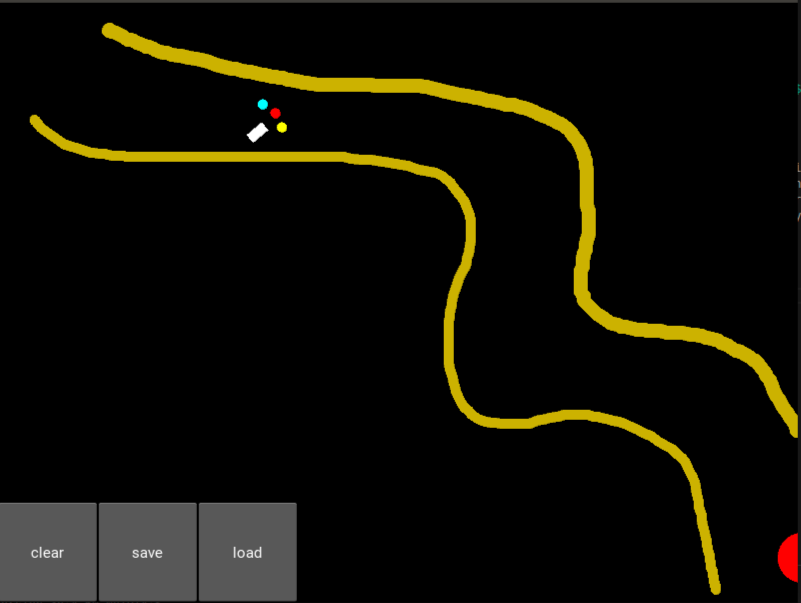
\includegraphics[width=0.4\textwidth]{imgs/simulator.png}
        \caption{\label{fig:simulation} Simulation of the system}
    \end{figure}


    As can be seen in the figure. The car is represented by a white square. The sonars of the car are represented by the three circles at the front of the car.
    
    \begin{figure}[!htb]
        \centering
        
\includegraphics[width=0.2\textwidth]{imgs/robot.png}
        \caption{\label{fig:simulation} Robot sonars}
    \end{figure}
    

    The walls are represented by the yellow lines. And the objective of the robot is represented by the red dot. 
    At first, the robot can cross walls but when it does so its speed decreases and it gets a negative reward because it has crossed the wall and because it will arrive less quickly at its target.


\section*{Proposed method}
The objective of our work is to train an agent to be able to choose the orientation angle of the car according to his perception of the environment. 

\subsection{network structure}

The structure of the network is quite simple. The network takes as input: 
the distances output by the sonars, and the angle formed by the direction of the robot and the line passing through the centre of the robot and target.
To simplify the teaching process, we have discretised the robot's exit space. The robot can make three decisions: do nothing, increment its angle by +20 degrees or -20 degrees.
Of course, making the exit area discreet means poorer results in the long term. But it allows for a quicker convergence towards a more stable policy \cite{Actor}.
    \begin{figure}[H]
        \centering
        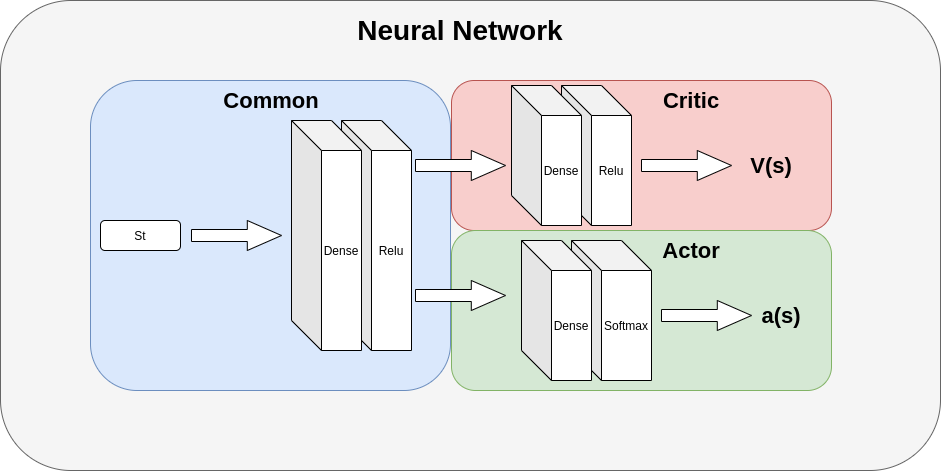
\includegraphics[width=0.5\textwidth]{imgs/network.png}
        \caption{\label{fig:method} Neural Network Structure}
    \end{figure}

As you can see the network is divided into two parts\cite{ANN}:
\begin{itemize}
    \item Critic 
    
    
    The Critic part is used to determine the value of the state in which the agent is in. 
    This part corresponds to the value-based part of the learning. It allows to stabilize the learning and to converge towards a global maximum of the policy.
    \item Actor
    
    
    The actor part corresponds to the part of the agent that takes action. It is the policy-based part of learning. 
    The actor part pulls out a probability distribution $\pi_{\theta}(s)$ which makes it possible to determine what probability is for the agent to take this or that action given the state.
  \end{itemize}
  The advantage of such a method is that a continuous space of action can be used.\cite{CONT}
  Unlike conventional Deep Q-Learning methods.\cite{DQN}
  The problem is that algorithms such as the DDPG (Deep deterministic policy gradient) which provide a continuous policy space do not guarantee to find the optimal policy for a given network and MDP, which is the case for a stochastic critical actor.
    Moreover, they introduce many problems that make them difficult to converge.\cite{DBLP}
    That's why we discretize the space in this problem.
    Here he purpose of learning is to change the probability distribution in the direction that gives the maximum reward. 

  The value part allows to compare the quality of an action carried out in relation to the value of a state already estimated to know if this action is more optimised than what has been done before.


\subsection{Advantage Actor Critic algorithm}

To update the network parameters we used reinforcement learning. We used one of the most powerful reinforcement learning algorithms before the A3C. A2C is an algorithm halfway between value based learning and policy based learning.
\begin{figure}[H]
    \centering
    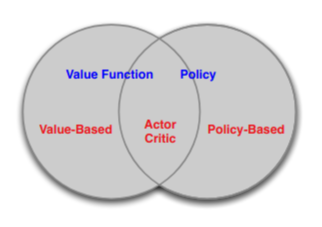
\includegraphics[width=0.3\textwidth]{imgs/actro.png}
    \caption{\label{fig:method} Actor Critic}
\end{figure}

The Advantage Actor Critic algorithm takes the following form :

\begin{figure}[H]
    \centering
    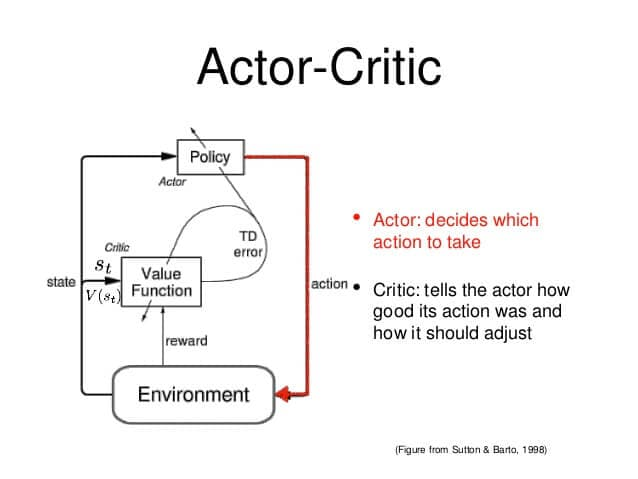
\includegraphics[width=0.5\textwidth]{imgs/actor_critic.jpeg}
    \caption{\label{fig:method} Actor Critic}
\end{figure}

\begin{algorithm}
\label{alga2c}
\caption{N-step Advantage Actor-Critic\label{a2c}}
\begin{algorithmic}[1]
\Procedure{N-Step Advantage Actor-Critic}{}
\State $\textit{Start with policy model } \pi_\theta \textit{ and value model } V_\omega$
\State $\textbf{repeat:}$
\State $\qquad\textit{Generate an episode } S_0, A_0, r_0, \ldots, S_{T-1}, A_{T-1}, r_{T-1} $
\State $\qquad\textbf{for } t \textit{ from } T-1 \textit{ to } 0$:
\State $\qquad\qquad V_{end} = 0 \text{ if } (t+N \geq T) \textit{ else } V_\omega(s_{t+N})$
\State $\qquad\qquad R_t =\gamma^{N}V_{end}+\sum_{k=0}^{N-1} \gamma^k \left(r_{t+k} \textit{ if } (t+k < T) \textit{ else } 0\right)$ 
\State $\qquad L(\theta) = \frac{1}{T} \sum_{i=0}^{T-1} (R_t - V_\omega(S_t)) \log \pi_\theta(A_t | S_t)$
\State $\qquad L(\omega) = \frac{1}{T} \sum_{i=0}^{T-1} (R_t - V_\omega(S_t))^2$
\State $\qquad\textit{Optimize } \pi_\theta \textit{ using } \nabla L(\theta)$
\State $\qquad\textit{Optimize } V_\omega \textit{ using } \nabla L(\omega)$
\EndProcedure
\end{algorithmic}
\end{algorithm}
As can be seen in figure 4, the principle of the critical actor is to take an action thanks to the actor and to criticise the action achieved thanks to the critic. But to criticise this action you need something to compare this action with the critic. This is the Advantage part. 
There are several ways of expressing Advantage.
But the most common method is to take as the advantage :  $Rt - V_{\pi_{\theta}(s,a)}$

with $Rt =\gamma^{N}V_{end}+\sum_{k=0}^{N-1} \gamma^k (r_{t+k})$.


We have used the Monte-Carlo evaluation.
The Monte-Carlo method involves letting an agent learn from the environment by interacting with it and collecting samples. This is equivalent to sampling from the probability distribution P(s, a, s’) and R(s, a).

However, Monte-Carlo (MC) estimation is only for trial-based learning. In other words, an MDP without the P tuple can learn by trial-and-error, through many repetitions.

In this learning process, each “try” is called an episode, and all episodes must terminate. That is, the final state of the MDP should be reached. Values for each state are updated only based on final reward Rt, not on estimations of neighbor states — as occurs in the Bellman Optimality Equation.

MC learns from complete episodes and is therefore only suitable for what we call episodic MDP.

Here it's not the case, but we are going to use the same method to take into account more information.

As can be seen in figure 5, the advantage part of the algorithm can also be called the TD error.

In the literature one initially finds $Rt =\gamma V_{t+1}+r_{t}$
but recent work on replay experience has shown that taking into account more rewards (like the monte-carlo evaluation) makes it easier to converge towards a global minimum of the cost function estimating the MDP (Markovian decision process).
On the other hand, using this method implies a certain volatility of the estimator since a stock affects the value of a state further in time, and it often takes longer to converge.
It is therefore a question of finding the best hyper-parameters, which are often found empirically.

\subsection{Reward process}
In reinforcement learning methods the reward process is very important as it allows the robot to perceive its environment. 
More importantly, it corresponds to the MRP (Markovian reward process) that we try to estimate thanks to the neural network (the critical part). 
So if the reward process does not correspond exactly to the environment, the agent will not correctly estimate the behaviour it has to adopt.
\begin{equation}
    \label{eqn:constrains}
    \begin{cases}
        R_{t}=-2,   \text{ if } None \text{(life penalty)}\\
        R_{t}=+1,   \text{ if } distance_{t}  <  distance_{t-1}\\
        R_{t}=-5,   \text{ if } x,y \in \Omega_{sand}\\

    \end{cases}
\end{equation}

The life penalty, allows the agent to get out of certain situations such as when he comes into contact with a wall and gets stuck. 
If a negative life penalty is not applied, the robot may get stuck in its situation.


\section*{Experimental discussion and results}
The neural network used is quite simple so the learning process is not long but the final results can be improved.
To evaluate the quality of a reinforcement learning project, it is not enough to look at the final quality of the model.
It is necessary to evaluate the training time, the response time of the system, and to determine on parameters such as the learning curve if the model can still learn or if it is not the case.

\subsection*{Learning}

It is difficult to visualize neural network learning for reinforcement learning problems.
Especially when using a critical actor.
In fact, if the error on the critic decreases it does not necessarily mean that the actor learns correctly. But it is really the actor who interests us. The error on the actor can be interpreted but it does not allow us to visualize the quality of the policy used by the agent at a given moment t.
To visualize the evolution of an agent in his environment, we must take into account the number of rewards he acquires over time.

\begin{figure}[H]
    \centering
    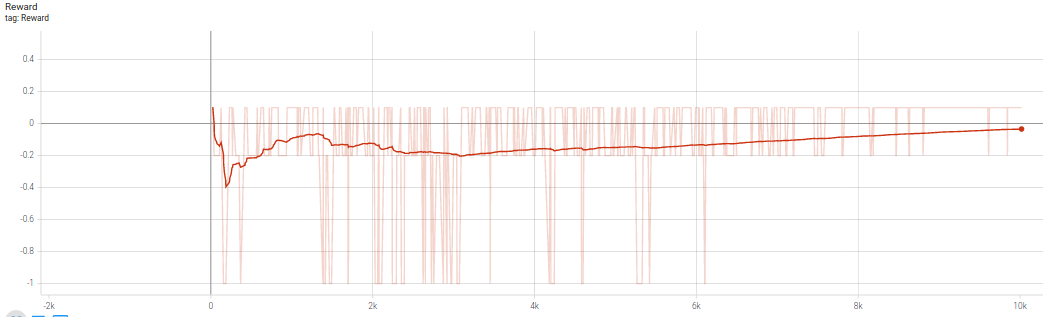
\includegraphics[width=0.5\textwidth]{imgs/reward.png}
    \caption{\label{fig:method} Rewards curve}
\end{figure}

As can be seen on the reward curve the model converges to an acceptable policy after 10K iterations, which is about 5 minutes.
We can consider that the model learned very quickly. 
The environment is quite simple since at first we don't use walls.

\subsection*{Obstacle avoidance}
Our initial goal was to create an agent capable of avoiding all the obstacles he could find.
With the chosen network and the established configuration our agent is able to reach his target avoiding most of the obstacles. 
\begin{figure}[H]
    \centering
    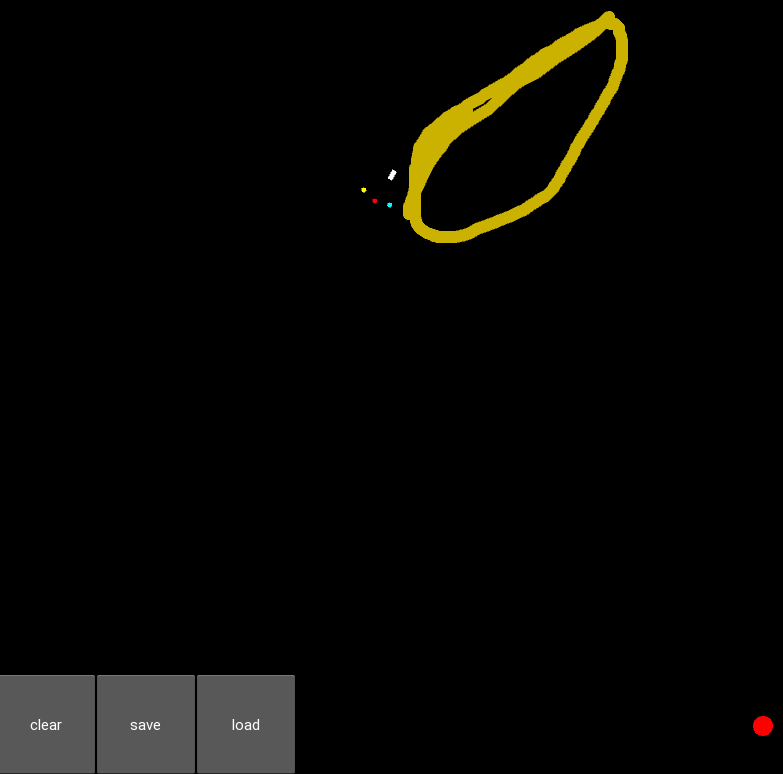
\includegraphics[width=0.1\textwidth]{imgs/obstacle.png}
    \caption{\label{fig:method} Avoiding one Obstacle}
\end{figure}
Even following a path.
\begin{figure}[H]
    \centering
    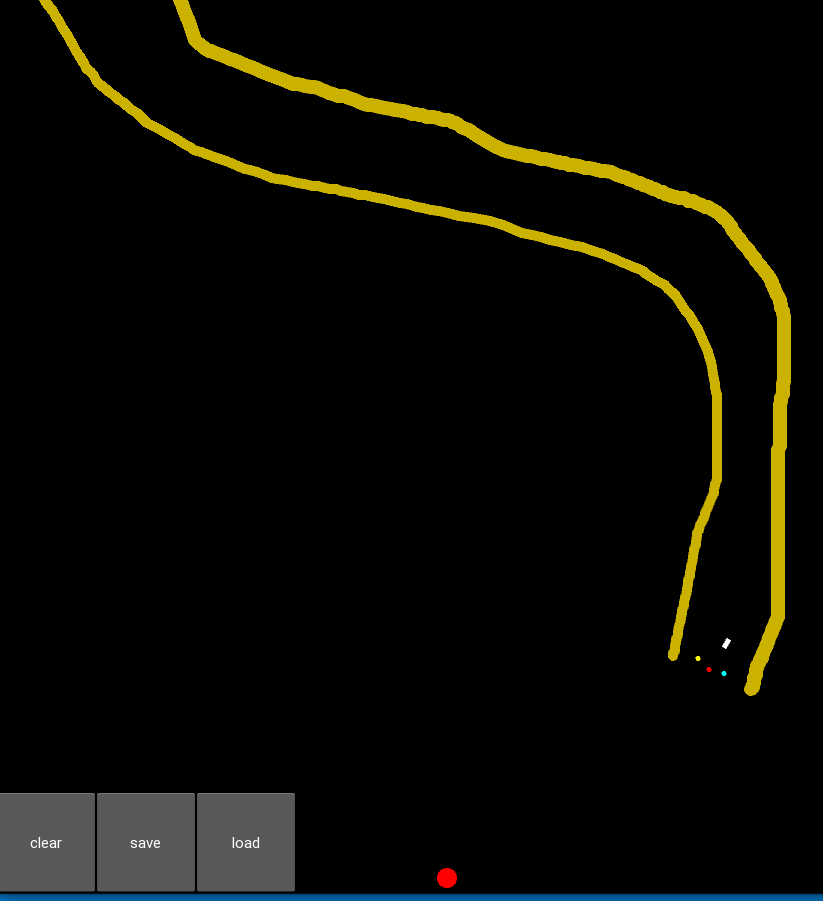
\includegraphics[width=0.1\textwidth]{imgs/path.png}
    \caption{\label{fig:method} Avoiding one Obstacle}
\end{figure}
However in some configurations the robot is sometimes forced to cross the wall to reach the target.
\begin{figure}[H]
    \centering
    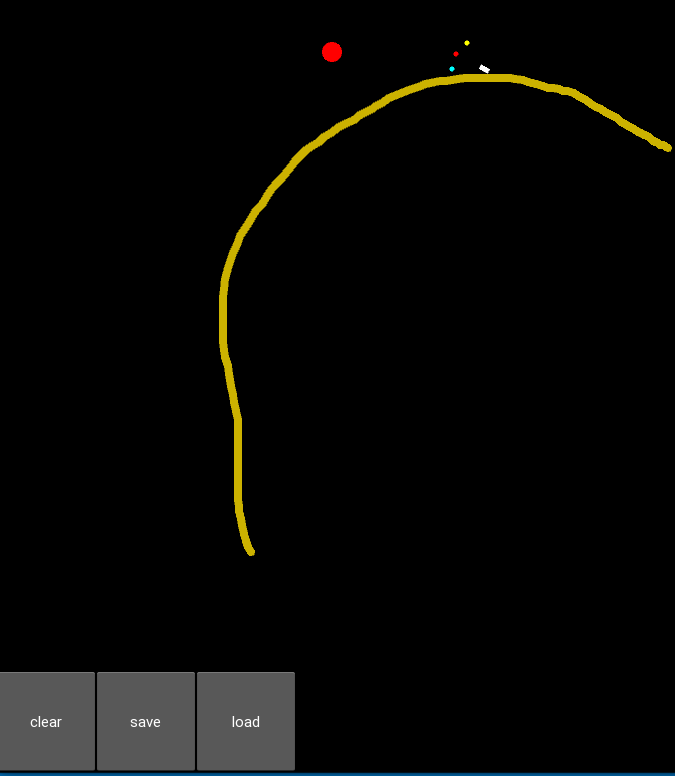
\includegraphics[width=0.1\textwidth]{imgs/U.png}
    \caption{\label{fig:method} The U problem.}
\end{figure}
So if the model presents very good results, it is still perfectible.
To check the results go to : \href{https://github.com/Paul-antoineLeTolguenec/Actor-critic}{Actor-Critic}.

\subsection*{Prospects for improvement}

As the results obtained are the result of a detailed search for the best hyper-parameters of the model (learning rate, gamma, etc.), there are three ways of improving the agent's performance:
\begin{itemize}
    \item \textbf{Building a deeper network}
    One of the possible reasons is that the network that has been built is not sufficient to find the most optimal policy in this Markovian decision process problem.
    One of the solutions is therefore to create a deeper network and thus to add layers of neurons.
    \item \textbf{Add an lstm layer} 
    LSTM \cite{LSTM} are recurrent neural networks. They make it possible to store information in memory. So in case the robot is stuck in a corner, it would be able to know where it comes from. For the moment it only goes with what it sees. Keeping information in memory could probably optimise the robot's performance.
    However, using this type of network leads to problems that can be difficult to solve, such as the vanishing gradient.\cite{vanishing}
    \item \textbf{Implementing another algorithm}
    As we have seen, there are several ways to train a neural network to find the CDM.
    But one of the most optimal methods is the A3C \cite{A3C} algorithm. (asynchronous  advantage  actor-critic)
    This method maximizes the exploration of several agents communicating with each other to find the best policy.
\end{itemize}


\section*{Conclusion}
Our method makes it possible to approximate the CDM and find an acceptable policy. However, the model can still learn. For the moment a more conventional method such as a vector field would work without any doubt.
But the advantage of reinforcement learning methods is that it can be applied to a totally different problem without changing the agent structure and therefore the method.
This is not the case with conventional methods where each problem introduces a new method.



%\section*{Sled localization}
    By having a box enclosing the trailing robot, and an interval framing the angle $x_4$, we are able to obtain a box containing the sled, knowing the length of the rope.
    
    This box has the shape of a pie sector. \textit{Equation}~\ref{eq:magnetometer} presents the position of the magnetometer as a function of the state of the system $x_1$, $x_2$ and $x_4$. Here all these variables are intervals. By applying a polar contractor to these intervals, we are able to obtain the intervals containing $x_m$ and $y_m$.

    \begin{equation}\label{eq:magnetometer}
        \left\lbrace
            \begin{aligned}
                x_m &= x_1 - L.cos(x_4) \\
                y_m &= x_2 - L.sin(x_4)
            \end{aligned}
        \right.
    \end{equation}

%\section*{Magnetometer range of measurement}
    By knowing a box containing the magnetometer and its measuring range, we are able to find all the points seen for sure and all the points that could be seen by the magnetometer. This allows us to recover the coverage of the area by the magnetometer.

    \begin{figure}[!htb]
        \centering
        \includegraphics[width=0.4\textwidth]{imgs/thickset_cmap.png}
        \caption{\label{fig:thickset} Measurement range of the magnetometer using Thicksets}
    \end{figure}

    The \textsc{Figure}~\ref{fig:thickset} shows us these two sets. The green set is the unseen area, the orange set is the area maybe seen and the red set is the area seen for sure by the magnetometer. The yellow set forms the uncertain boundary between the other sets, which can be adjusted. Thus we have a way to know precisely the coverage of the mapping during the mission.

%\section*{Magnetometer Mapping}
    With a moving box enclosing the magnetometer at any time, this method allows us to recover the coverage of the area by the magnetometer. Thus we have a way to know precisely the coverage of the mapping during the mission, which depends on the uncertainty on the position of the magnetometer and on the maximum distance of each point of the field to be measured. An example of the covered area of a magnetometer on a field is presented by the \textsc{Figure}~\ref{fig:thickset_trajectory}.

    \begin{figure}[!htb]
        \centering
        \includegraphics[width=0.4\textwidth]{imgs/thickset_fine_cmap.png}
        \caption{\label{fig:thickset_trajectory} Coverage of the map by the magnetometer using Thicksets}
    \end{figure}
    

%\section*{Application example}
    In this part we will see on a practical case what we are able to do with this implementation. We place ourselves in the same conditions as before, i.e. we are in the case of a magnetometer dragged by a robot with tank type evolution equations and the rope must remain tight all along the mission.

    Here we want our robot to follow the following Lissajous trajectory:

    \begin{empheq}[left={\forall t \in \mathbb{R}, \qquad \mathcal{T}(t) = }\empheqlbrace]{align}
        x(t) &= 20\times sin\left(\frac{2\times t}{20}\right) \\
        y(t) &= 20\times sin\left(\frac{3\times t}{20}\right)
    \end{empheq}

    \begin{empheq}[left={\forall t \in \mathbb{R}, \qquad \frac{d\mathcal{T}(t)}{dt} = }\empheqlbrace]{align}
        \frac{dx(t)}{dt} &= 2\times cos\left(\frac{2\times t}{20}\right) \\
        \frac{dy(t)}{dt} &= 3\times cos\left(\frac{3\times t}{20}\right)
    \end{empheq}

    \begin{empheq}[left={\forall t \in \mathbb{R}, \qquad \frac{d^2\mathcal{T}(t)}{dt^2} = }\empheqlbrace]{align}
        \frac{d^2x(t)}{dt^2} &= -\frac{4}{20}\times sin\left(\frac{2\times t}{20}\right) \\
        \frac{d^2y(t)}{dt^2} &= -\frac{9}{20}\times sin\left(\frac{3\times t}{20}\right)
    \end{empheq}

    \begin{figure}[!htb]
        \centering
        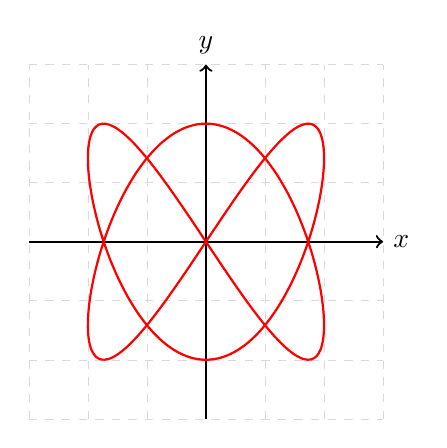
\begin{tikzpicture}[scale=1.5]
            \draw[help lines, color=gray!30, dashed, step=0.5] (-1.5,-1.5) grid (1.5,1.5);
            \draw[->,thick] (-1.5,0)--(1.5,0) node[right]{$x$};
            \draw[->,thick] (0,-1.5)--(0,1.5) node[above]{$y$};
            \draw[color=red,thick,domain=0:500, smooth, samples=150] plot ({sin(2*\x},{sin(3*\x)});
        \end{tikzpicture}
        \caption{Lissajous trajectory}
    \end{figure}

    The \textit{control.py} file is able to generate the controls to drive the trailing robot. These commands are generated by feedback linearization by controlling the robot in speed and heading. These controls leads to the trajectory in the simulator  as we could see on the \textsc{Figure}~\ref{fig:simulator_lissajous}

    \begin{figure}
        \centering
        \includegraphics[width=0.4\textwidth]{imgs/simulator_lissajous.png}
        \caption{Simulator's trajectory of the system}
        \label{fig:simulator_lissajous}
    \end{figure}

    Then the module \textit{mapping.py} allows to process the tubes including the trajectory of the trailing robot and the sledge. The tubes are then displayed in order to check that they seem to stick to the trajectory of the system.

    \begin{figure}[!htb]
        \centering
        \includegraphics[width=0.4\textwidth]{imgs/saturne_lissajous.png}
        \caption{Trailing vehicle enclosing tube}
        \label{fig:saturne_lissajous}
    \end{figure}

    \begin{figure}[!htb]
        \centering
        \includegraphics[width=0.4\textwidth]{imgs/magnetometer_lissajous.png}
        \caption{Magnetometer enclosing tube}
        \label{fig:magnetometer_lissajous}
    \end{figure}

    \begin{figure}[!htb]
        \centering
        \includegraphics[width=0.4\textwidth]{imgs/mapping_lissajous.png}
        \caption{Magnetometer enclosing tube}
        \label{fig:mapping_lissajous}
    \end{figure}

% \begin{acknowledgements}
% \blindtext
% \end{acknowledgements}

% \section*{Bibliography}
% \bibliography{zHenriquesLab-Mendeley}

% %% You can use these special %TC: tags to ignore certain parts of the text.
% %TC:ignore
% %the command above ignores this section for word count
% \onecolumn
% \newpage

% \section*{Word Counts}
% This section is \textit{not} included in the word count. 
% \subsection*{Notes on Nature Methods Brief Communication}
% \begin{itemize}
% \item Abstract: 3 sentences, 70 words.
% \item Main text: 3 pages, 2 figures, 1000-1500 words, more figures possible if under 3 pages
% \end{itemize}

% \subsection*{Statistics on word count}
% \detailtexcount
% \newpage

%%%%%%%%%%%%%%%%%%%%%%%%%%%%%
% Supplementary Information %
%%%%%%%%%%%%%%%%%%%%%%%%%%%%%
% \captionsetup*{format=largeformat}
% \section{Something about something} \label{note:Note1} 
% \Blindtext

%TC:endignore
%the command above ignores this section for word count

\end{document}